\begin{frame}{The Essential Problem: Poor Sampling of Feature Space}
\begin{tikzpicture}[scaleall=1.0]
\pcuad{\textwidth}{\textheight}
\path(nw) ++(-1,-0.5) node(graphic1)[anchor=north west]{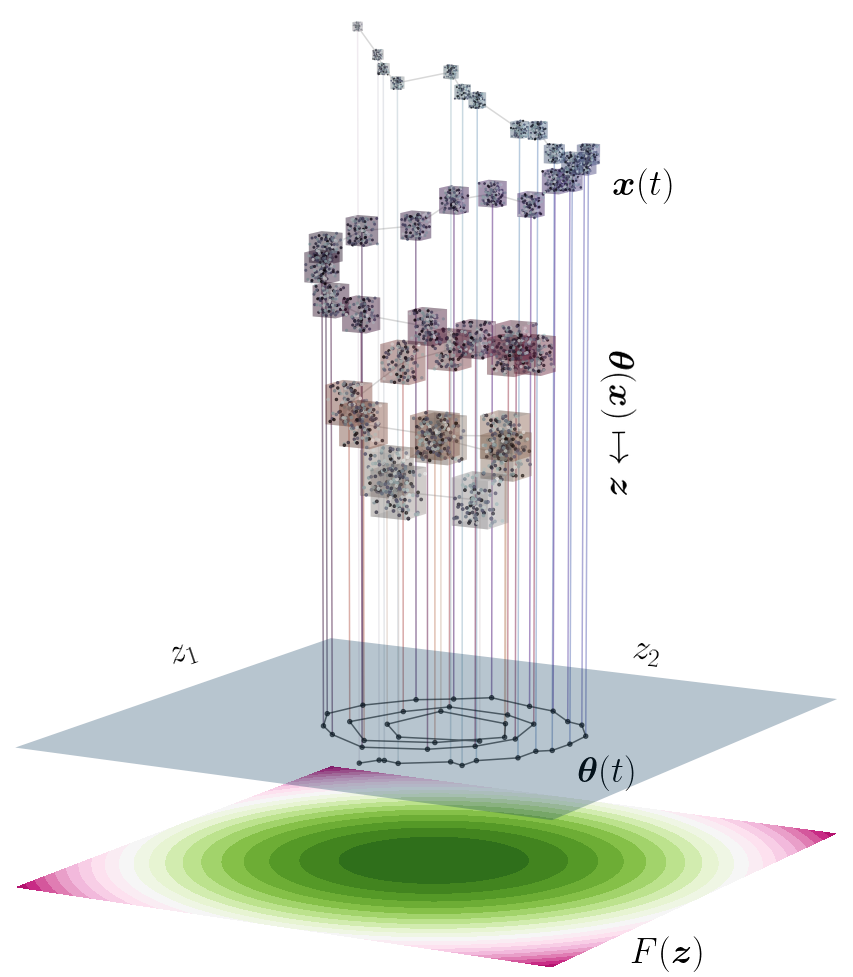
\includegraphics[width=0.6\textwidth]{hmmdfig-crop.png}};
\path(np) ++(-1,0) node(line1)[anchor=north west]{Configuration space $\xb^{3N} \equiv [(x_0,x_1,x_2)_1,\dots]$}
          ++(0,-1) node(line2)[anchor=west]{MD: $m_i\ddot{x}_i = -\nabla_iV(\xb) + \mbox{ensemble forces}$}
          ++(1,-1) node(line3)[anchor=west]{Samples $\Rightarrow\ \xb(t_1),\ \xb(t_2),\ \dots$}
          ++(0,-1) node(line4)[anchor=west]{Ergodicity: $\displaystyle\langle X\rangle \approx \frac{1}{n_\tau}\sum_{i=1}^{n_\tau} X[\xb(t_i)]$}
          ++(-1.3,-1) node(line5)[anchor=west]{Mapping configuration space}
          ++(0,-0.4) node(line5)[anchor=west]{to feature space}
          ++(0.25,-1.) node(line6)[anchor=west]{Feature space: $\zb^M \equiv (z_1,z_2,\dots)$}
          ++(0,-2) node(line7)[anchor=west]{Free energy: $F(\zb)=-k_{\rm B}T\ln\langle\delta\left[\theta(\xb)-\zb\right]\rangle$};
\end{tikzpicture}
\end{frame}
